\documentclass[journal]{IEEEtran}

\usepackage{amsmath}
\usepackage{balance}
\usepackage{booktabs}
\usepackage{cite}
\usepackage{stfloats}
\usepackage{tabularx}
\usepackage{tikz}
\usepackage{xspace}
\usepackage[hidelinks]{hyperref}
\usetikzlibrary{arrows.meta,positioning}

\newcommand{\project}{\textsc{CHIA-RDO}\xspace}
\newcommand{\metric}[1]{\textbf{#1}}

\definecolor{softblue}{HTML}{EAF3FA}
\definecolor{deepblue}{HTML}{245A7A}
\definecolor{softpurple}{HTML}{F1ECF8}
\definecolor{deeppurple}{HTML}{665080}
\definecolor{softorange}{HTML}{FFF1DE}
\definecolor{deeporange}{HTML}{A65F18}
\definecolor{softgreen}{HTML}{EAF6EC}
\definecolor{deepgreen}{HTML}{347447}
\definecolor{softred}{HTML}{FBECEC}
\definecolor{deepred}{HTML}{9A4545}

\tikzset{
  block/.style={draw=black,rounded corners=1pt,align=center,
                minimum height=5.5mm,inner xsep=2pt,font=\scriptsize},
  hw/.style={block,double,double distance=0.4pt},
  result/.style={block,thick},
  flow/.style={-{Latex[length=1.6mm]},draw=black},
  feedback/.style={-{Latex[length=1.6mm]},draw=black,dashed}
}

\title{From HM-Side Adaptive $K$ to Variable-$K$ RTL:\\
A CHIA Loop for HEVC RDO Co-Design}

\author{Nguyen Hieu Duong and Duy Hieu Bui\\
\normalsize Vietnam National University\\
\normalsize Corresponding author: 24020497@vnu.edu.vn\\
\footnotesize Artifact: \url{https://github.com/duongnguyenhieu/CHIA-RDO},
release \texttt{chia-rdo-v1.0.0}}

\markboth{A3 CHIA Hackathon Final Submission, 2026}%
{Duong and Bui: From HM-Side Adaptive $K$ to Variable-$K$ RTL}

\begin{document}
\maketitle

\begin{abstract}
HEVC intra coding exposes 35 luma prediction modes, making full
rate--distortion optimization (RDO) expensive. \project separates the resulting
co-design problem into two explicit implementations. Patched HM-16.20 software
ranks all 35 modes and selects $K\in\{4,16,35\}$ from normalized rough cost;
the RTL receives that already-ranked prefix and does not implement pruning,
rough mode decision, or CABAC bit estimation. Its hardware contribution is a
variable-$K$ batch scheduler, 16 serial 4$\times$4 candidate-evaluation lanes,
and stable balanced winner reduction. The frozen HM-side policy reduces
held-out candidate RDO evaluations by \metric{38.21\%} while retaining
\metric{97.91\%} of Full-RDO winners; aggregate Y-PSNR BD-rate is $-0.026\%$ on
the limited corpus. Physical feedback replaces monolithic candidate logic and
a linear winner scan, yielding a routed kernel at a derived
\metric{68.120 MHz} and \metric{8.134 M candidates/s}, 2.128$\times$ the P1
baseline proxy. A CHIA loop preserves the software contract while independently
searching and verifying this RTL microarchitecture.
\end{abstract}

\begin{IEEEkeywords}
Agentic co-design, adaptive candidate selection, FPGA, HEVC, rate--distortion
optimization, RTL.
\end{IEEEkeywords}

\section{Introduction and Background}
\IEEEPARstart{H}{igh} Efficiency Video Coding (HEVC) improves compression by
evaluating a large set of spatial prediction choices, but this flexibility
makes intra-mode search computationally expensive. For each prediction unit,
the HM reference encoder first applies rough mode decision (RMD), using SATD
and an estimated signaling cost to rank 35 luma modes. It then performs the
more expensive rate--distortion optimization (RDO), which reconstructs and
compares shortlisted candidates using distortion and coded-rate estimates
\cite{hm1620}.

Fast intra-decision methods reduce this workload by pruning candidates before
full RDO. Fixed-size shortlists are simple but cannot adapt to content: smooth
or strongly directional blocks may need few candidates, whereas textured or
ambiguous blocks benefit from broader search. Prior adaptive methods use
features such as relative SATD and statistical risk to trade encoding effort
for coding efficiency \cite{gwon2019}. These methods are usually evaluated as
software algorithms, without considering how each candidate budget maps to a
parallel hardware scheduler.

That mapping creates a cross-layer problem. An FPGA with $P$ lanes executes
$\lceil K/P\rceil$ batches, so two policies with equal mean $K$ can incur
different latency and lane utilization. Conversely, increasing $P$ can reduce
batches while increasing area, routing pressure, and critical-path delay.
Algorithm selection and RTL architecture therefore need a shared evidence loop
rather than independent optimization.

\project addresses this gap without claiming that the pruning policy itself is
hardware. It connects software coding quality, cycle-accurate RTL correctness,
and routed physical feedback while preserving a precise boundary between them.
Its principal contributions are:
\begin{enumerate}
  \item a frozen \emph{HM-side} Adaptive-$K$ policy and matched coding curves;
  \item an explicit event contract carrying the selected $K$, stable rank,
        HM bit counts, QP, lambda, references, and original samples into RTL;
  \item a variable-$K$ RTL architecture whose scheduler, serial candidate
        lanes, and balanced stable-argmin differ from fixed-size or
        cost-only candidate arrays; and
  \item a CHIA graph preserving RTL tests, routed feedback, cache behavior,
        and Pareto history for replay and claim auditing.
\end{enumerate}

\section{HM-Side Adaptive-$K$ Algorithm}
\textbf{Software responsibility.} Every operation in this section executes in
patched HM-16.20, not in SystemVerilog. The policy treats a low normalized best
rough cost as evidence that one mode already predicts the block well, so a
short expensive-RDO prefix is sufficient; ambiguous blocks retain more
candidates. For each luma PU, HM:
\begin{enumerate}
  \item computes
  $C[m]=\mathrm{SATD}[m]+\mathrm{bits}[m]\sqrt{\lambda}$ for every mode
  $m=0,\ldots,34$;
  \item stable-sorts modes by increasing $C$, retaining lower mode ID on an
  exact tie;
  \item computes
  \begin{equation}
    \widehat C_{\min}=\frac{\min_m C[m]}{WH(2^b-1)},
  \end{equation}
  for PU size $W\!\times\!H$ and luma bit depth $b$;
  \item selects
  \begin{equation}
  K=\begin{cases}
      4,  & \widehat C_{\min}\le 0.04,\\
      16, & 0.04<\widehat C_{\min}\le 0.20,\\
      35, & \widehat C_{\min}>0.20;
    \end{cases}
  \end{equation}
  \item runs candidate RDO on exactly the first $K$ ranked modes, retaining
  the earlier stable rank on an exact RD-cost tie.
\end{enumerate}

\textbf{Difference from other selection rules.} Fixed-$K$ always evaluates the
same prefix. Our relative-SATD baseline instead counts modes within a relative
SATD threshold and rounds that count to an allowed $K$. The selected rule uses
only the absolute best signaling-aware rough cost, normalized by PU area and
sample range; it needs neither a trained Bayesian classifier nor subset
statistics. It is not a reproduction of Gwon--Choi \cite{gwon2019}. A bounded
discovery comparison selected $(0.04,0.20;4,16,35)$ below a predeclared 1\%
BD-rate gate; its identity was then frozen before held-out evaluation.

For coding experiments, HM executes candidate RDO on the first $K$ ranks. For
RTL regression, HM additionally exports each candidate's integer bit count and
floating-point lambda; the vector bridge rounds lambda to Q16.16 and packages
an event. The policy deliberately excludes lane count $P$, scheduler state,
QP, and activity. Hardware latency follows only afterward as
$\lceil K/P\rceil$ batches, so RTL exploration cannot change the selected
prefix. This artifact is a software-to-vector/test flow, not a live HM--FPGA
integration. Matched curves use pinned HM-16.20, Main 8-bit 4:2:0 All-Intra,
four frames, and QP 22/27/32/37.

\section{End-to-End Co-Design Architecture}
\begin{figure*}[!t]
\centering
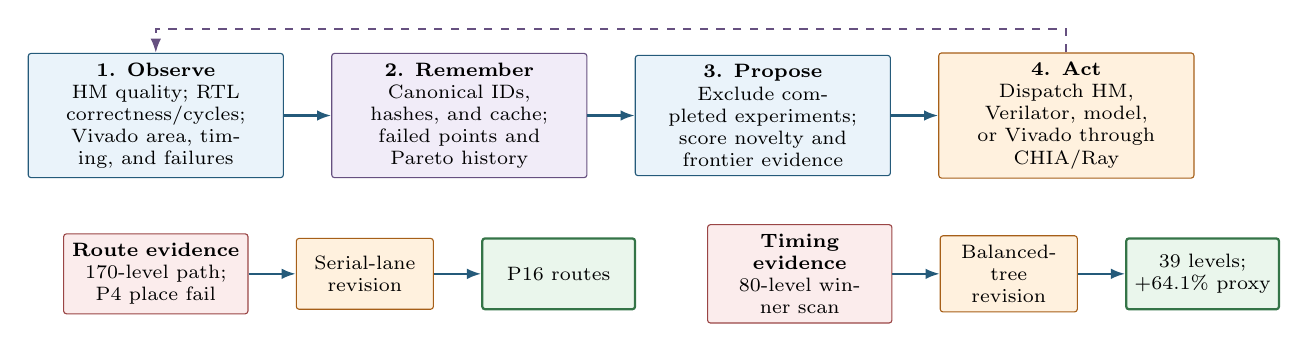
\begin{tikzpicture}[
  node distance=3mm and 6mm,
  phase/.style={block,text width=31mm,minimum height=15mm,font=\scriptsize},
  evidence/.style={block,text width=22mm,minimum height=9mm,font=\scriptsize,
                   draw=deepred,fill=softred},
  revision/.style={block,text width=16mm,minimum height=9mm,font=\scriptsize,
                   draw=deeporange,fill=softorange},
  outcome/.style={block,text width=18mm,minimum height=9mm,font=\scriptsize,
                  draw=deepgreen,fill=softgreen,thick},
  agentflow/.style={-{Latex[length=1.8mm]},draw=deepblue,thick},
  agentfeedback/.style={-{Latex[length=1.8mm]},draw=deeppurple,thick,dashed}
]
  \node[phase,draw=deepblue,fill=softblue] (observe)
    {\textbf{1. Observe}\\HM quality; RTL correctness/cycles;\\Vivado area, timing, and failures};
  \node[phase,right=of observe,draw=deeppurple,fill=softpurple] (memory)
    {\textbf{2. Remember}\\Canonical IDs, hashes, and cache;\\failed points and Pareto history};
  \node[phase,right=of memory,draw=deepblue,fill=softblue] (propose)
    {\textbf{3. Propose}\\Exclude completed experiments;\\score novelty and frontier evidence};
  \node[phase,right=of propose,draw=deeporange,fill=softorange] (act)
    {\textbf{4. Act}\\Dispatch HM, Verilator, model,\\or Vivado through CHIA/Ray};
  \draw[agentflow] (observe)--(memory);
  \draw[agentflow] (memory)--(propose);
  \draw[agentflow] (propose)--(act);
  \draw[agentfeedback] (act.north) -- ++(0,3mm) -| (observe.north);

  \node[evidence,below=7mm of observe] (ev1)
    {\textbf{Route evidence}\\170-level path; P4 place fail};
  \node[revision,right=of ev1] (rev1) {Serial-lane\\revision};
  \node[outcome,right=of rev1] (out1) {P16 routes};
  \node[evidence,right=9mm of out1] (ev2)
    {\textbf{Timing evidence}\\80-level winner scan};
  \node[revision,right=of ev2] (rev2) {Balanced-tree\\revision};
  \node[outcome,right=of rev2] (out2) {39 levels;\\+64.1\% proxy};
  \foreach \a/\b in {ev1/rev1,rev1/out1,ev2/rev2,rev2/out2}
    \draw[agentflow] (\a)--(\b);
\end{tikzpicture}
\caption{The history-aware agentic loop and two concrete evidence-to-action
traces. The controller proposes experiments; each versioned RTL revision then
re-enters the same verification and backend loop.}
\label{fig:loop}
\end{figure*}

Here \emph{agentic} denotes a closed observe--remember--propose--act loop, not an
LLM that emits unchecked RTL. Native \texttt{ChiaFunction} nodes dispatch tools
asynchronously. Typed results expose quality, correctness, cycle, resource,
timing, and failure signals; atomic records preserve canonical experiment IDs,
source hashes, successful and failed points, and Pareto history. The
deterministic proposal policy removes completed IDs, rewards underexplored
configurations and frontier boundaries, and gives promoted RTL measurements
priority. Track A rejects any mutation of the frozen Adaptive-$K$ identity.

Actions remain auditable: the controller selects and dispatches experiments,
while each source-level microarchitectural revision is versioned before it
re-enters regression and routing. Thus Fig.~\ref{fig:loop} does not claim
autonomous RTL generation; it shows how remembered backend evidence changes
the next design hypothesis. The campaign accumulated 114 history records, 107
successful logical experiments, 11 matched HM curves, and a 10-point Pareto
set. A calibrated graph then screened 832 $P$/depth/width combinations and
produced 16 Pareto points; replay returned 832/832 cache hits without rerunning
tools. The HM branch measures policy quality, whereas Verilator/Vivado evaluate
only the contracted kernel, so agentic exploration cannot move Adaptive-$K$
across the boundary in Fig.~\ref{fig:rtl}.

\section{Hardware Algorithm and RTL Architecture}
\textbf{Not implemented in RTL:} 35-mode RMD, stable sorting, the threshold
test that chooses $K$, lambda derivation, and CABAC-context bit estimation.
\textbf{Implemented in RTL:} variable-$K$ dispatch, complete 4$\times$4 luma
candidate arithmetic for each supplied rank, fixed-point RD cost, and stable
winner selection. This distinction is the central hardware/software contract.

A start transaction supplies $K$; up to 35 ranked 6-bit modes and aligned
24-bit rate counts; 6-bit QP; 32-bit $\lambda$; seventeen 8-bit top/left
references; and the row-major 4$\times$4 8-bit original luma block. The final
\texttt{full\_rdo\_pway\_optimized} elaboration uses $P=16$, depth 3, and a
31-bit cost. Its ready/valid scheduler dispatches candidate $bP+l$ to lane $l$
and masks the partial final batch.

\begin{figure}[!b]
\centering
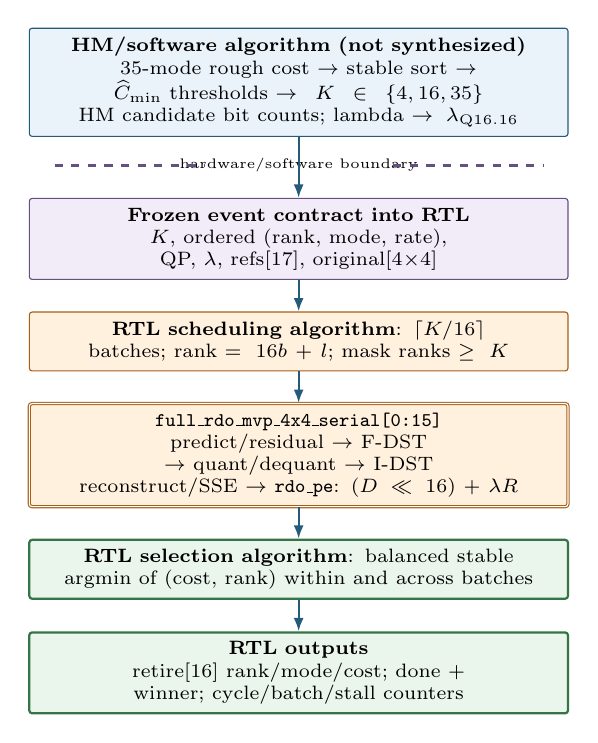
\begin{tikzpicture}[
  node distance=4mm,
  swstage/.style={block,text width=67mm,draw=deepblue,fill=softblue},
  contract/.style={block,text width=67mm,draw=deeppurple,fill=softpurple},
  rtlstage/.style={block,text width=67mm,draw=deeporange,fill=softorange},
  selectstage/.style={block,text width=67mm,draw=deepgreen,fill=softgreen,thick},
  archflow/.style={-{Latex[length=1.7mm]},draw=deepblue,thick}
]
  \node[swstage] (sw) {\textbf{HM/software algorithm (not synthesized)}\\
    35-mode rough cost $\rightarrow$ stable sort $\rightarrow$
    $\widehat C_{\min}$ thresholds $\rightarrow K\in\{4,16,35\}$\\
    HM candidate bit counts; lambda $\rightarrow\lambda_{\mathrm{Q16.16}}$};
  \node[font=\tiny,below=1.5mm of sw] (boundary) {hardware/software boundary};
  \draw[deeppurple,dashed,thick] ([xshift=-31mm]boundary.center)--([xshift=-12mm]boundary.center);
  \draw[deeppurple,dashed,thick] ([xshift=12mm]boundary.center)--([xshift=31mm]boundary.center);
  \node[contract,below=2mm of boundary] (event) {\textbf{Frozen event contract into RTL}\\
    $K$, ordered (rank, mode, rate), QP, $\lambda$, refs[17], original[4$\times$4]};
  \node[rtlstage,below=of event] (sched)
    {\textbf{RTL scheduling algorithm}: $\lceil K/16\rceil$ batches;
    rank $=16b+l$; mask ranks $\ge K$};
  \node[rtlstage,double,double distance=0.4pt,below=of sched] (lanes)
    {\texttt{full\_rdo\_mvp\_4x4\_serial[0:15]}\\
    predict/residual $\rightarrow$ F-DST $\rightarrow$ quant/dequant $\rightarrow$ I-DST\\
    reconstruct/SSE $\rightarrow$ \texttt{rdo\_pe}: $(D\ll16)+\lambda R$};
  \node[selectstage,below=of lanes] (tree)
    {\textbf{RTL selection algorithm}: balanced stable argmin of (cost, rank)
    within and across batches};
  \node[selectstage,below=of tree] (outputs) {\textbf{RTL outputs}\\
    retire[16] rank/mode/cost; done + winner; cycle/batch/stall counters};
  \foreach \a/\b in {sw/event,event/sched,sched/lanes,lanes/tree,tree/outputs}
    \draw[archflow] (\a)--(\b);
\end{tikzpicture}
\caption{Algorithm partition and selected RTL. Adaptive-$K$ ends above the
boundary; hardware preserves its ranked prefix while evaluating candidates and
selecting the winner. Each serial lane takes 132 cycles per candidate.}
\label{fig:rtl}
\end{figure}

The scheduler differs from fixed-$K$ hardware by accepting any event count up
to 35, preserving input rank, and masking the last partial batch. It differs
from a cost-only array because each lane computes prediction through SSE rather
than receiving distortion. Within a lane, one sample or coefficient is advanced
per FSM cycle, replacing the earlier monolithic combinational candidate path.
Across lanes, a balanced tree replaces the earlier 16-way linear winner scan.
The comparison is lexicographic: lower cost wins, then lower supplied rank.
Per-lane retirement exposes rank/mode/cost; event completion also returns the
winner and cycle, batch, stall, and lane-activity counters. A no-backpressure
batch retires in 134 cycles.

\begin{figure}[!t]
\centering
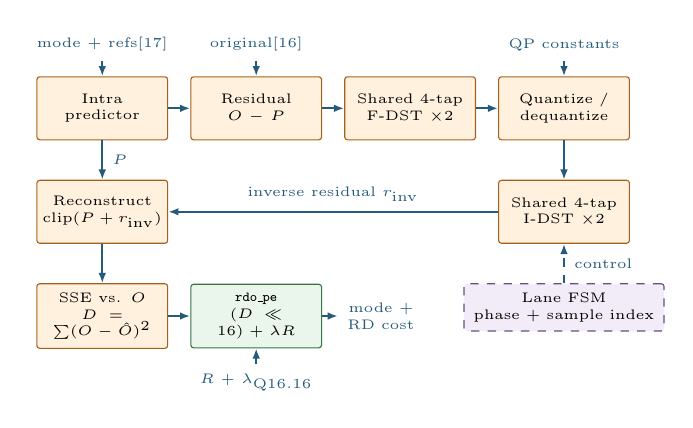
\begin{tikzpicture}[
  node distance=5mm and 2.8mm,
  lane/.style={block,text width=15.2mm,minimum height=8mm,font=\tiny,
               draw=deeporange,fill=softorange},
  datum/.style={font=\tiny,align=center,text=deepblue},
  control/.style={block,dashed,text width=24mm,minimum height=6mm,font=\tiny,
                  draw=deeppurple,fill=softpurple},
  tinyflow/.style={-{Latex[length=1.3mm]},draw=deepblue,thick}
]
  \node[lane] (pred) {Intra\\predictor};
  \node[lane,right=of pred] (res) {Residual\\$O-P$};
  \node[lane,right=of res] (fdst) {Shared 4-tap\\F-DST $\times2$};
  \node[lane,right=of fdst] (quant) {Quantize /\\dequantize};
  \node[lane,below=of quant] (idst) {Shared 4-tap\\I-DST $\times2$};
  \node[lane,below=of pred] (recon) {Reconstruct\\clip$(P+r_{\mathrm{inv}})$};
  \node[lane,below=of recon] (sse) {SSE vs. $O$\\$D=\sum(O-\hat O)^2$};
  \node[lane,right=of sse,draw=deepgreen,fill=softgreen] (rd)
    {\texttt{rdo\_pe}\\$(D\ll16)+\lambda R$};

  \draw[tinyflow] (pred)--(res);
  \draw[tinyflow] (res)--(fdst);
  \draw[tinyflow] (fdst)--(quant);
  \draw[tinyflow] (quant)--(idst);
  \draw[tinyflow] (idst.west)--node[datum,above] {inverse residual $r_{\mathrm{inv}}$}
    (recon.east);
  \draw[tinyflow] (pred)--node[datum,right] {$P$} (recon);
  \draw[tinyflow] (recon)--(sse);
  \draw[tinyflow] (sse)--(rd);

  \node[datum,above=2mm of pred] (refs) {mode + refs[17]};
  \node[datum,above=2mm of res] (orig) {original[16]};
  \node[datum,above=2mm of quant] (qp) {QP constants};
  \node[datum,below=2mm of rd] (rate) {$R$ + $\lambda_{\mathrm{Q16.16}}$};
  \node[datum,right=2mm of rd] (cost) {mode +\\RD cost};
  \draw[tinyflow] (refs)--(pred);
  \draw[tinyflow] (orig)--(res);
  \draw[tinyflow] (qp)--(quant);
  \draw[tinyflow] (rate)--(rd);
  \draw[tinyflow] (rd)--(cost);

  \node[control,below=of idst] (fsm)
    {Lane FSM\\phase + sample index};
  \draw[tinyflow,dashed] (fsm)--node[datum,right] {control} (idst);
\end{tikzpicture}
\caption{Candidate datapath inside one serial RTL lane. This is bounded HEVC
4$\times$4 arithmetic, not the Adaptive-$K$ policy. Registers between phases
store 16 intermediate samples while arithmetic is reused across positions;
16 identical lanes feed the stable reduction tree in Fig.~\ref{fig:rtl}.}
\label{fig:lane}
\end{figure}

\subsection{Verification Evidence}
Final campaigns executed 121,600 vector/candidate checks. The depth-3 serial
corpus alone contains 8,960 vectors covering all 35 modes and four QPs; the
tree campaign adds 10,560 P1/P8/P16 evaluations including backpressure. Stage
values, order, winners, cycle counts, dropped/duplicate checks, and interfaces
all passed with zero failures.

\section{Software-Algorithm and RTL Evaluation}
\begin{table*}[!t]
\caption{Coding Results Relative to the Full-RDO Anchor}
\label{tab:coding}
\centering
\footnotesize
\setlength{\tabcolsep}{3.5pt}
\begin{tabularx}{\textwidth}{@{}>{\raggedright\arraybackslash}p{0.21\textwidth}
  >{\raggedright\arraybackslash}X r r r r@{}}
\toprule
\textbf{Method / Corpus} & \textbf{Candidate Rule} & \textbf{Avg. $K$} &
\textbf{RDO Red.} & \textbf{Retention} & \textbf{BD-Rate} \\
\midrule
Full-RDO anchor & All 35 rough-ranked modes & 35.000 & 0.00\% & 100.00\% & 0.000\% \\
Fixed-$K$8 / discovery & First 8 ranked modes & 8.000 & 77.14\% & 68.05\% & +3.574\% \\
Relative-SATD / discovery & Threshold count, quantized $K$ & 25.624 & 26.79\% & 96.07\% & +0.528\% \\
Frozen threshold / discovery & Normalized rough cost; $K=4/16/35$ & 18.651 & 46.71\% & 90.25\% & +0.755\% \\
Fixed-$K$16 / held-out & First 16 ranked modes & 16.000 & 54.29\% & 85.70\% & +0.016\% \\
\textbf{Frozen threshold / held-out} & \textbf{Same policy, no retuning} &
\textbf{21.628} & \textbf{38.21\%} & \textbf{97.91\%} & \textbf{$-$0.026\%} \\
HW-aware Track-B / P8 & Joint quality/cycle objective & 16.456 & 52.98\% & 88.02\% & $-$0.054\% \\
\bottomrule
\end{tabularx}
\par\vspace{2pt}
\footnotesize RDO reduction is $1-\mathrm{Avg.}K/35$; retention is the fraction
of blocks whose Full-RDO winner remains in the prefix. Negative aggregate
BD-rate on three synthetic held-out families is not a general quality claim.
\end{table*}

The direct held-out comparison exposes the software-algorithm tradeoff:
Fixed-$K$16 prunes more work, but loses the Full-RDO winner on 14.30\% of
blocks; Adaptive-$K$ spends extra candidates on ambiguous content and lowers
that loss to 2.09\%. It removes only 13.95\% and 13.30\% of evaluations on
mixed-texture and repetitive families, but 87.36\% on smooth/edge content.
Track-B is separately versioned and does not alter the frozen policy.

The Gwon--Choi relative-SATD Bayesian method reports 31.54\% average encoding
time reduction and +0.93\% BD-rate against HM-16.6 under its own Intra Main
condition \cite{gwon2019}. It starts from stock-HM RMD modes and includes a
minimum-risk Bayesian classifier. Our relative-SATD baseline instead starts
from all 35 modes and uses threshold counting only, so the published result is
context rather than a direct comparison.

\section{RTL Evolution from Physical Feedback}
The first P-way baseline replicated a monolithic candidate datapath. At P1,
the critical path traversed prediction, residual, both forward-transform
passes, quant/dequant, both inverse passes, reconstruction, and distortion:
170 logic levels, including 69 CARRY8 levels. P2 reached 175 levels, and P4
exceeded LUT/CARRY capacity before placement.

The next proposal serialized work within each lane and inserted state
boundaries between major arithmetic phases. This raised Fmax and reduced
per-lane area, allowing P16 to route, but a serial 16-way winner scan became an
80-level path. The final balanced tree reduced that path; the routed critical
path is now 39 levels inside one lane's prediction/residual datapath and ends
at a residual-sample RAM input.

\subsection{Measured Interpretation}
To compare routed variants under a common 5 ns constraint, we report
\begin{equation}
 f_{\mathrm{derived}}=\frac{1}{5\,\mathrm{ns}-\mathrm{WNS}},\qquad
 T_{\mathrm{kernel}}=\frac{P f_{\mathrm{derived}}}{C_{\mathrm{batch}}}.
\end{equation}
This post-route comparison proxy is distinct from encoder frames/s. The
selected P16 design routes with WNS $=-9.680$ ns, hence
$f_{\mathrm{derived}}=68.120$ MHz and $T_{\mathrm{kernel}}=8.134$ M
candidates/s for 134-cycle batches.

\subsection{Resource Budget}
On the KV260 device (117,120 LUTs, 1,248 DSPs), the final design uses 52.26\%
of LUTs and 65.38\% of DSPs. Against the project's 70\%-of-device integration
budget, this is 74.66\% of the LUT allowance and 93.47\% of the DSP allowance,
leaving 57 DSPs. P16 is the throughput endpoint of the Pareto frontier, not the
minimum-area or minimum-power point.

\section{Routed Microarchitecture Comparison}
\begin{table}[!t]
\caption{Routed Implementations}
\label{tab:routed}
\centering
\scriptsize
\setlength{\tabcolsep}{1.8pt}
\begin{tabularx}{\columnwidth}{@{}>{\raggedright\arraybackslash}X r r r r r@{}}
\toprule
\textbf{Architecture} & \textbf{$P$} & \textbf{LUT/DSP} & \textbf{WNS} &
\textbf{MHz} & \textbf{M/s} \\
\midrule
Mono. combinational & 1 & 36,454/178 & $-$60.395 & 15.292 & 3.823 \\
Mono. combinational & 2 & 70,817/356 & $-$64.653 & 14.357 & 7.178 \\
Serial d3, w31 & 8 & 30,813/408 & $-$9.620 & 68.399 & 4.084 \\
Serial P16 scan & 16 & 60,232/816 & $-$19.092 & 41.508 & 4.956 \\
\textbf{Serial P16 tree} & \textbf{16} & \textbf{61,207/816} &
\textbf{$-$9.680} & \textbf{68.120} & \textbf{8.134} \\
\bottomrule
\end{tabularx}
\par\vspace{1pt}
\scriptsize All rows routed. WNS is in ns; MHz is derived from the routed
critical path; M/s is the candidate-kernel rate.
\end{table}

The balanced tree costs 975 LUTs and 45 FFs over the P16 serial scan, leaves
DSP count unchanged, and reduces estimated power from 2.338 W to 2.288 W. It
improves derived Fmax by 64.1\% and kernel rate by 64.1\%. Relative to the
monolithic P1 proxy, its candidate rate is 2.128$\times$; relative to P2 it is
1.133$\times$. The calibrated CHIA model predicts P16 within 0.14\% for LUT,
0.45\% for Fmax/throughput, and 0.43\% for power.

\section{Reproducibility and Deliverables}
Local/GCP parity produced identical bitstream, reconstruction, and trace hashes
for a reference encode. GCP workers later replayed RTL campaigns with zero
failures. Post-run Compute Engine queries found no remaining instances, disks,
or reserved addresses. Actual billed spend and promotional-credit balance
remain unavailable and are not replaced by estimates.

The artifact preserves policy versions, manifests, source and corpus hashes,
raw Vivado reports, machine-readable result schemas, and Pareto history.
Principal deliverables are CHIA proposal/evaluation graphs and the deterministic
policy controller; pinned HM patches, matched quality curves, and synthetic
fixtures; parameterized SystemVerilog, golden vectors, and Verilator campaigns;
and analytical replay, model calibration, routed reports, and parsers.

\balance
\section{Limitations and Next Step}
The coding study uses small deterministic synthetic All-Intra workloads, not
standard natural-video classes. RTL is limited to 4$\times$4 8-bit luma and
excludes chroma, inter prediction, larger transforms, RDOQ, syntax coding, and
hardware CABAC/context evolution. Exact HM candidate bit counts are supplied
externally. The 31-bit cost width is corpus-qualified, not formally bounded for
arbitrary input. Most importantly, this artifact does not connect a running HM
encoder directly to the FPGA: software selects and packages each event, and
RTL begins only at the interface in Fig.~\ref{fig:rtl}.

Resource scale is also a limitation. The selected design uses 816 DSP48E2
primitives, exactly 51 per lane times 16 lanes. ``Serial'' describes candidate
execution within a lane; it does not imply one shared multiplier. Runtime
products in prediction, quant/dequant, squared error, and the 24$\times$32-bit
$\lambda R$ term infer multiple DSP slices, and the RTL does not explicitly
share these multipliers across lanes. The P16 scan already uses 60,232 LUTs;
the balanced tree adds 975 LUTs and 45 FFs but no DSPs, producing the
61,207-LUT total. A final hierarchical utilization split by operation was not
preserved, so finer DSP attribution would require a new synthesis report.

All physical runs are out of context and omit board-level clocks, pins, AXI,
and encoder integration. The routed result is therefore reported using its
derived critical-path frequency. Future work will pipeline forward-transform
accumulation and repeat regression, routing, and board-level integration.

Within these limits, \project demonstrates the intended agentic co-design
behavior: it preserves a software-quality contract, searches reproducibly,
checks a bit-exact kernel, and uses failed backend evidence to produce a
specific microarchitectural revision rather than merely requesting more
parallelism.

\begin{thebibliography}{4}
\bibitem{chia2026}
CHIA, ``An open framework for agile and principled hardware/software co-design
research,'' arXiv:2606.27350, 2026.

\bibitem{gwon2019}
D. Gwon and H. Choi, ``Relative SATD-based minimum risk Bayesian framework for
fast intra decision of HEVC,'' \emph{KSII Trans. Internet Inf. Syst.}, vol. 13,
no. 1, pp. 385--405, Jan. 2019, doi: 10.3837/tiis.2019.01.022.

\bibitem{hm1620}
ITU-T/ISO/IEC, ``High Efficiency Video Coding Test Model HM-16.20.''

\bibitem{artifact}
\project artifact. [Online]. Available:
\url{https://github.com/duongnguyenhieu/CHIA-RDO}, release
\texttt{chia-rdo-v1.0.0}.
\end{thebibliography}

\noindent\footnotesize AI assistance was used in preparing this artifact.

\end{document}
